\chapter{Quantum correlations in the weakly-interacting Bose gas}

\NOTE{TOUT CECI EST MAL ECRIT}

One of the key and on-going challenges of quantum mechanics is to understand macroscopic systems containing a large number of particles $N$, commonly referred as many-body physics. Trying to consider all the possible degrees of freedom of each individual particle and interactions effects would result in an incredibly complex problem impossible to solve theoretically. Studying such systems thus require to use approximations ...

Physicists were able to describe a gas of a large number of bosonic particles with increasing complexity throughout history. The first step was the development of statistical physics, aiming to build a bridge between the microscopic properties of individual atoms or molecules and macroscopic properties of bulk materials described by thermodynamics. This approach culminated in the theory of the ideal Bose gas, ideal meaning here that all particles are non-interacting. This theory found great success with the notable prediction of a new state of matter, the Bose-Einstein condensate. 

The next step was then to increase the complexity of the problem by adding interactions between the particles. ...

While also greatly successful, the mean-field approach neglects by essence interaction phenomena between individual particles. To characterize such effects, we thus need to go beyond the mean-field approximation. \NOTE{c'est bien nul je laisse pour l'instant}




\section{Correlation functions}

\subsection{First order correlation function of light}

Let us begin our journey with correlation functions with the simple example of the classical description of light. Correlation functions of light were developed in strong connection with the notion of \textbf{coherence} characterizing the possibility for waves to interfere. A light field is said to be coherent when there is a fixed phase relationship for the electric field at different positions (spatial coherence) and different times (time coherence). 


\begin{figure}
    \centering
    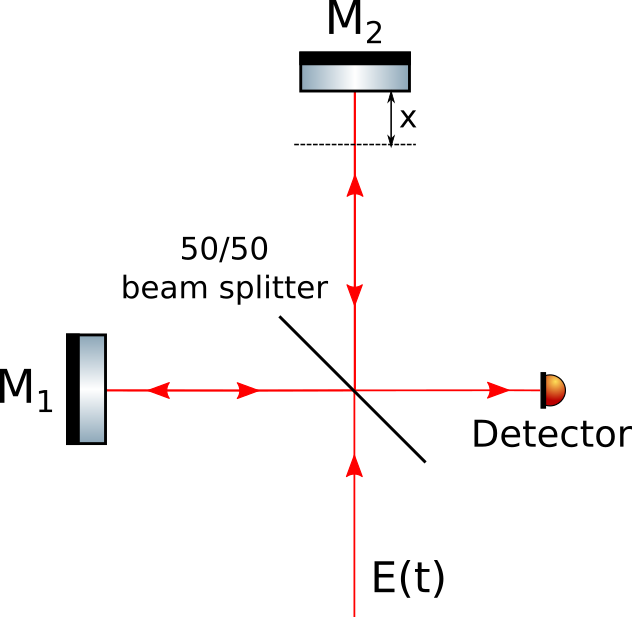
\includegraphics[width=0.55\textwidth]{Fig/Chapter1/michelson.png}
    \caption{Principle of the Michelson interferometer.}
    \label{fig:michelson}
\end{figure}


To illustrate where correlation functions come from, let us begin by taking a look at time coherence in the emblematic Michelson interferometer (see Fig.-\ref{fig:michelson}). We send at the input of the interferometer a complex light field $E(t)$. The intensity measured by the detector writes:

\begin{equation}
    I=\mean{\abs{E(t)+E(t-\tau)}^2}
    \label{eq:i_michelson}
\end{equation}

where $\mean{...}$ denotes the time average made by the detector and $\tau=\frac{2x}{c}$ the delay between the two interfering waves induced by the optical path difference between the two arms of the interferometer. Developing equation \ref{eq:i_michelson} we get:

\begin{equation}
    I=\mean{\abs{E(t)}^2} + \mean{\abs{E(t-\tau)}^2} + 2 {\rm{Re}} \mean{E(t) E^*(t-\tau)}
\end{equation}

For simplicity sake, let's assume that the source is stationary to write $\mean{\abs{E(t)}^2} = \mean{\abs{E(t-\tau)}^2} = I_0$, we then obtain :

\begin{equation}
    I= 2 I_0 (1 + {\rm{Re}} (g^{(1)} (\tau))) \ , \ g^{(1)} (\tau) = \frac{ \mean{E(t) E^*(t-\tau)}}{\mean{\abs{E}^2}}
\end{equation}

We have introduced the normalized \textbf{first-order correlation function} $g^{(1)}$ that characterizes the interference term. If $E(t)$ and $E(t-\tau)$ are independent and thus uncorrelated, $\mean{E(t) E^*(t-\tau)} = \mean{E(t)} \mean{ E^*(t-\tau)}=0$ and interference cannot be observed \NOTE{corriger}. On the other hand, if there is a \textbf{correlation} between these two quantities, an interference phenomenon can be observed. The same reasoning can be conducted for the spatial coherence for instance with the non less famous Young double slit experiment. 

We will not detail here all the intricacies of the study of first-order correlation functions for different light sources. The main point to remember is that the first order correlation function is a natural way to characterize the coherence properties of a light source, and thus its ability to produce interferences. 





\subsection{Classical example : HBT with chaotic light}

\subsection{HBT with the perfect Bose gas}

\section{Bogoliubov theory of the weakly-interacting gas}

Thus far, we have familiarized ourselves with correlation functions and seen through a few examples the kind of information they contain. We will now try to use this tool to study a many-body problem, the weakly-interacting homogeneous Bose gas, {\it i.e.} an ensemble of bosonic particles with weak contact interactions in a box of volume $V$. The theoretical description of this system has been developed by Nikolay Bogoliubov in his famous 1947 article \cite{bogoliubov1947}. In this section, we will remind the main lines of Bogoliubov's approach and see what it tells us in terms of correlation functions.

\subsection{Bogoliubov approximation}

\NOTE{Etapes avant?}

The Hamiltonian of the weakly-interacting Bose gas with contact interactions writes:

\begin{equation}
    \hat{H}=\sum_{\bm{k}}\frac{\hbar^2 k^2}{2m} \hat{a}^{\dagger}_{\bm{k}}  \hat{a}_{\bm{k}} +  \frac{g}{2V} \sum \hat{a}^{\dagger}_{\bm{k_1}+\bm{k_3}} \hat{a}^{\dagger}_{\bm{k_2}-\bm{k_3}} \hat{a}_{\bm{k_1}} \hat{a}_{\bm{k_2}} 
\end{equation}

\noindent where $g=\dfrac{4 \pi \hbar^2 a_s}{m}$ is the strength of the interactions with $a_s$ the s-wave sacttering length. \NOTE{DILUTENESS?} In order to simplify this Hamiltonian, we use the Bogoliubov approximation that relies on two points:

\begin{itemize}
    \item Since the interactions are weak, we assume that the number of atoms outside of the BEC is small. We therefore only consider interaction processes removing two particles from the BEC or bringing back two particles into the BEC. Mathematically speaking, we drop all terms higher than quadratic in $\hat{a}_{\bm{k}}$ and $\hat{a}^{\dagger}_{\bm{k}}$.
    \item The number of atoms $\NBEC$ is assumed to be very large. Therefore, we replace $\hat{a}_{\bm{0}}$ and $\hat{a}^{\dagger}_{\bm{0}}$ by $\sqrt{\NBEC}$. 
\end{itemize}

With these approximation, the simplified Hamiltonian writes:

\begin{equation}
    H_{\rm{bogo}}=\sum_{\bm{k}}\frac{\hbar^2 k^2}{2m} a^{\dagger}_{\bm{k}}  a_{\bm{k}} +  \frac{g\NBEC}{2V} \sum_{\bm{k}} (a^{\dagger}_{\bm{k}} a^{\dagger}_{-\bm{k}} +a_{\bm{k}} a_{-\bm{k}})+\frac{g\NBEC^2}{2V}
\end{equation}

What we now want to is diagonalize the Hamiltonian. This is achieved through the linear Bogoliubov transformation where we introduce a new operator:

\begin{equation}
    \hat{b}_{\bm{k}}=u_{\bm{k}} \hat{a}_{\bm{k}} + v_{-\bm{k}} \hat{a}^{\dagger}_{-\bm{k}}
\end{equation}

To determine the expression of the coefficients $u_{\bm{k}}$ and $v_{\bm{k}}$, we impose that the new operator $\hat{b}_{\bm{k}}$ follows the bosonic operator commutation rule:

\begin{equation}
    [\hat{b}_{\bm{k}},\hat{b}^{\dagger}_{\bm{k}'}]= \delta_{\bm{k},\bm{k}'}
\end{equation}

This gives $u_{\bm{k}}^2 -  v_{-\bm{k}}^2 =1$. We can therefore write $u_{\bm{k}}={\rm cosh}(\alpha_{\bm{k}})$ and $v_{-\bm{k}}={\rm sinh}(\alpha_{\bm{k}})$ and look to determine $\alpha_{\bm{k}}$. This value must be chosen \NOTE{BLAH} giving:

\begin{equation}
    \frac{g n}{2}\left(u_{\bm{k}}^{2}+v_{-\bm{k}}^{2}\right)+\left(\frac{k^{2}}{2 m}+g n\right) u_{\bm{k}} v_{-\bm{k}}=0
\end{equation}

from which finally obtain:

\begin{equation}
    u_{\bm{k}}, v_{-\bm{k}}=\pm\left(\frac{\hbar^2k^{2} / 2 m+g n}{2 \varepsilon(k)} \pm \frac{1}{2}\right)^{1 / 2}
\end{equation}

with 

\begin{equation}
    \varepsilon(p)=\sqrt{\left[\frac{g n}{m} \hbar^2 k^{2}+\left(\frac{\hbar^2 k^{2}}{2 m}\right)^{2}\right]}
\end{equation}

the famous Bogoliubov dispersion relation.


\subsection{Spectrum of excitations}

\subsection{The quantum depletion}

\section{HBT with interacting atoms}

\section{k/-k correlations in the many-body ground-state}